\documentclass[
11pt, % The default document font size, options: 10pt, 11pt, 12pt
%codirector, % Uncomment to add a codirector to the title page
]{charter} 




% El títulos de la memoria, se usa en la carátula y se puede usar el cualquier lugar del documento con el comando \ttitle
\titulo{Sistema de monitoreo de un equipo de extracción de petróleo} 

% Nombre del posgrado, se usa en la carátula y se puede usar el cualquier lugar del documento con el comando \degreename
%\posgrado{Carrera de Especialización en Sistemas Embebidos} 
\posgrado{Carrera de Especialización en Internet de las Cosas} 
%\posgrado{Carrera de Especialización en Intelegencia Artificial}
%\posgrado{Maestría en Sistemas Embebidos} 
%\posgrado{Maestría en Internet de las cosas}

% Tu nombre, se puede usar el cualquier lugar del documento con el comando \authorname
\autor{Ing. Eduardo Agustín Sciutto} 

% El nombre del director y co-director, se puede usar el cualquier lugar del documento con el comando \supname y \cosupname y \pertesupname y \pertecosupname
\director{Mag. Ing. Adrián S. Nowik}
\pertenenciaDirector{UP/PAE} 
% FIXME:NO IMPLEMENTADO EL CODIRECTOR ni su pertenencia
\codirector{John Doe} % para que aparezca en la portada se debe descomentar la opción codirector en el documentclass
\pertenenciaCoDirector{FIUBA}

% Nombre del cliente, quien va a aprobar los resultados del proyecto, se puede usar con el comando \clientename y \empclientename
\cliente{Ing. Nicolás D. Brunini}
\empresaCliente{PAE}

% Nombre y pertenencia de los jurados, se pueden usar el cualquier lugar del documento con el comando \jurunoname, \jurdosname y \jurtresname y \perteunoname, \pertedosname y \pertetresname.
\juradoUno{Nombre y Apellido (1)}
\pertenenciaJurUno{pertenencia (1)} 
\juradoDos{Nombre y Apellido (2)}
\pertenenciaJurDos{pertenencia (2)}
\juradoTres{Nombre y Apellido (3)}
\pertenenciaJurTres{pertenencia (3)}
 
\fechaINICIO{21 de junio de 2022}		%Fecha de inicio de la cursada de GdP \fechaInicioName
\fechaFINALPlan{9 de agosto de 2022} 	%Fecha de final de cursada de GdP
\fechaFINALTrabajo{21 de junio de 2023}	%Fecha de defensa pública del trabajo final


\begin{document}

\maketitle
\thispagestyle{empty}
\pagebreak


\thispagestyle{empty}
{\setlength{\parskip}{0pt}
\tableofcontents{}
}
\pagebreak


\section*{Registros de cambios}
\label{sec:registro}


\begin{table}[ht]
\label{tab:registro}
\centering
\begin{tabularx}{\linewidth}{@{}|c|X|c|@{}}
\hline
\rowcolor[HTML]{C0C0C0} 
Revisión & \multicolumn{1}{c|}{\cellcolor[HTML]{C0C0C0}Detalles de los cambios realizados} & Fecha      \\ \hline
0      & Creación del documento                                 &\fechaInicioName \\ \hline
1      & Se completa hasta el punto 5 inclusive                 & 2 de julio de 2022 \\ \hline
2      & Se completa hasta el punto 9 inclusive					& 9 de julio de 2022 \\
\hline
3      & Se completa hasta el punto 12 inclusive				& 17 de julio de 2022 \\
\hline
4     & Se completa hasta el punto 15 inclusive				& 29 de julio de 2022 \\
\hline
5     & Se completa el plan				& 4 de agosto de 2022 \\
\hline
%		  Se puede agregar algo más \newline
%		  En distintas líneas \newline
%		  Así                                                    & dd/mm/aaaa \\ \hline
%3      & Se completa hasta el punto 11 inclusive                & dd/mm/aaaa \\ \hline
%4      & Se completa el plan	                                 & dd/mm/aaaa \\ \hline
\end{tabularx}
\end{table}

\pagebreak



\section*{Acta de constitución del proyecto}
\label{sec:acta}

\begin{flushright}
Buenos Aires, \fechaInicioName
\end{flushright}

\vspace{2cm}

Por medio de la presente se acuerda con el \authorname\hspace{1px} que su Trabajo Final de la \degreename\hspace{1px} se titulará ``\ttitle'', consistirá esencialmente en la implementación de un prototipo de un sistema de monitoreo de un equipo de extracción de petróleo, y tendrá un presupuesto preliminar estimado de 614 hs de trabajo y ARS 2.162.300,00, con fecha de inicio \fechaInicioName\hspace{1px} y fecha de presentación pública \fechaFinalName.

Se adjunta a esta acta la planificación inicial.

\vfill

% Esta parte se construye sola con la información que hayan cargado en el preámbulo del documento y no debe modificarla
\begin{table}[ht]
\centering
\begin{tabular}{ccc}
\begin{tabular}[c]{@{}c@{}}Dr. Ing. Ariel Lutenberg \\ Director posgrado FIUBA\end{tabular} & \hspace{2cm} & \begin{tabular}[c]{@{}c@{}}\clientename \\ \empclientename \end{tabular} \vspace{2.5cm} \\ 
\multicolumn{3}{c}{\begin{tabular}[c]{@{}c@{}} \supname \\ Director del Trabajo Final\end{tabular}} \vspace{2.5cm} \\
%\begin{tabular}[c]{@{}c@{}}\jurunoname \\ Jurado del Trabajo Final\end{tabular}     &  & \begin{tabular}[c]{@{}c@{}}\jurdosname\\ Jurado del Trabajo Final\end{tabular}  \vspace{2.5cm}  \\
%\multicolumn{3}{c}{\begin{tabular}[c]{@{}c@{}} \jurtresname\\ Jurado del Trabajo Final\end{tabular}} \vspace{.5cm}                                                                     
\end{tabular}
\end{table}




\section{1. Descripción técnica-conceptual del proyecto a realizar}
\label{sec:descripcion}


% El bloque "consigna" se usa para poner texto en rojo y dar una pequeña ayuda sobre cómo completar la sección

La gestión eficiente de un yacimiento productor de petróleo no electrificado y de periferia plantea grandes desafíos. El modelo de operación usualmente se basa en la presencia diaria de cuadrillas de operarios cuya principal función es recorrer cada instalación y realizar un relevamiento funcional. Excepcionalmente, ejecutan alguna tarea correctiva en función de lo identificado en la visita.
En la actualidad, existen zonas donde los aparatos individuales de bombeo (AIB) no disponen de supervisión remota dado que originalmente la implementación de una solución tradicional de telemetría fue considerada económicamente inviable. La principal razón, es el costo de proveer un sistema alternativo de energía confiable para dicho equipamiento que generalmente está basado en paneles solares y baterías. Otra consideración es el riesgo de sabotaje y robo de equipamiento de medición costoso en zonas alejadas y con vigilancia deficiente. 

El hecho de que un AIB deje de funcionar de manera imprevista, afecta directamente la producción de petróleo, por lo que resulta de valor disponer de una alerta inmediata ante dicha situación. Además, la información histórica de los períodos de tiempo de no funcionamiento facilita y hace más precisa la elaboración del informe de down-time por parte de los supervisores de producción.
 
Recientemente, la empresa operadora del yacimiento implementó una red LoRaWAN propia con extensa cobertura en el yacimiento. Sintéticamente, LoRaWAN es una tecnología de comunicación inalámbrica bidireccional, que hace posible administrar muchos nodos alimentados a baterías (con vida útil típica de varios años) conectados hasta varios kilómetros de distancia y transmitiendo a una muy baja tasa de datos (decenas de bytes pocas veces al día). Estas características hacen viable una implementación de internet de las cosas industrial (IIoT) para el caso mencionado, resaltando el aporte de mayor eficiencia y de reducción de costos operativos.

Otro aspecto para considerar es el de buscar una solución de rápida implementación y de mayor flexibilidad ante cambios, que aporte información relevante a los usuarios finales. Implementar un sistema de SCADA con tecnología tradicional es un trabajo complejo y demandante de tiempo, requiere la intervención de profesionales de distintos sectores dentro de la empresa ya que involucra tareas de configuración, calibración y enrutamiento en distintos sistemas on-premise. En muchos casos es justificada su utilización dada la criticidad e importancia de los procesos que se controlan y monitorean. Por otro lado, se ve una oportunidad en la utilización de distintos servicios en la nube, principalmente para procesar fuentes de datos no críticos que complementan o brindan nueva información de variables de campo y que se adaptan fácilmente a los cambios en las necesidades de visualización y notificación de los usuarios finales.

El objeto del presente proyecto es el desarrollo de una solución de monitoreo y alarmas de bajo costo para equipos AIB de un yacimiento de periferia. Se utilizarán una red LoRaWAN y componentes en la nube de Microsoft Azure.
En particular, se implementará un prototipo que medirá el estado funcional del AIB. El servidor de red LoRaWAN canalizará la información generada por el sensor a un grupo de recursos creados en la nube de Microsoft Azure mediante el protocolo AMQP.
En la nube se realizarán diferentes procesos, que contemplan la decodificación de la información, almacenamiento en base de datos y utilización de una aplicación back end que administrará el acceso a información estadística y la notificación de alertas a los usuarios autorizados.
Los usuarios dispondrán de al menos un tipo de front end para el consumo de la información.

En la figura \ref{fig:diagBloques} se presenta el diagrama en bloques del sistema descripto.

%\vspace{25px}

\begin{figure}[htpb]
\centering 
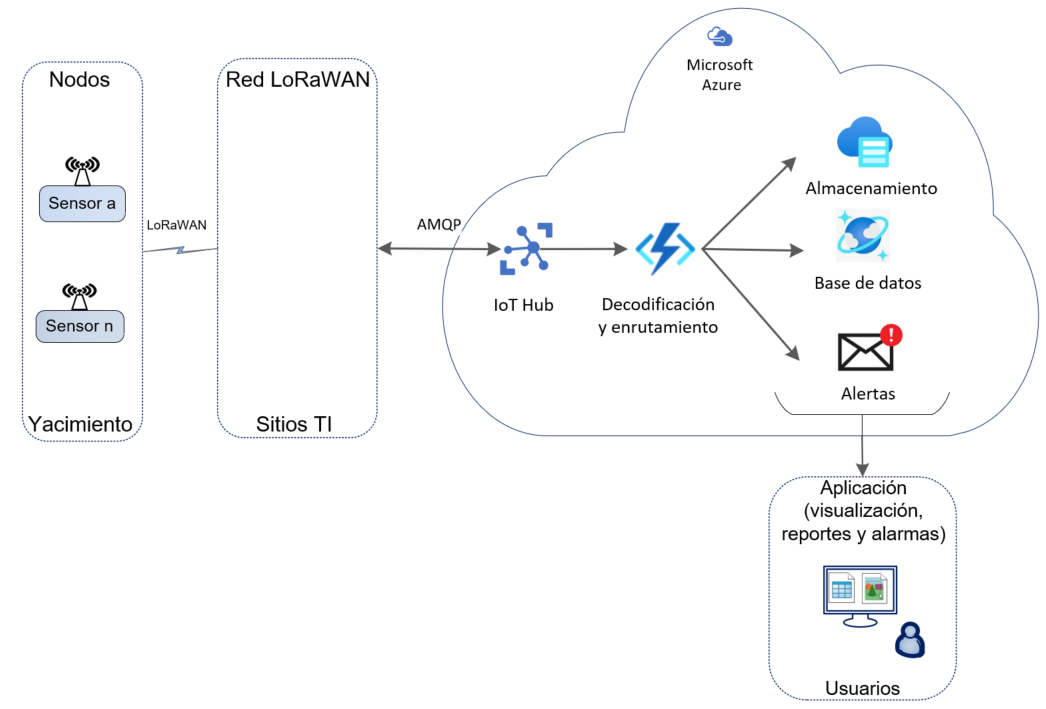
\includegraphics[width=.8\textwidth]{./Figuras/diagrama_bloques_conceptual2.png}
\caption{Diagrama en bloques del sistema.}
\label{fig:diagBloques}
\end{figure}

\vspace{25px}




\section{2. Identificación y análisis de los interesados}
\label{sec:interesados}


\begin{table}[ht]
%\caption{Identificación de los interesados}
%\label{tab:interesados}
\begin{tabularx}{\linewidth}{@{}|l|X|X|l|@{}}
\hline
\rowcolor[HTML]{C0C0C0} 
Rol           & Nombre y Apellido & Organización 	& Puesto 	\\ \hline
Auspiciante   & Juan A. Aranguren & \empclientename & Exec. Manager TEC-IT       	\\ \hline
Cliente       & \clientename      &\empclientename &  Leader UPO-OP II D5      	\\ \hline
Impulsor      & Eduardo O. Domínguez                  &\empclientename & Exec. Manager IT Regional       	\\ \hline
Responsable   & \authorname       &\empclientename        	& SR Specialist TEC-IT 	\\ \hline
Colaboradores & Gustavo G. Conrad \newline 
				Germán Gornatti					&\empclientename             	& Specialist TEC-IT  \\ \hline
%			& Germán Gornatti &\empclientename & SR Engineer UPO-Control Engineering     \\ \hline
Orientador    & \supname	      & \pertesupname 	& Director Trabajo final \\ \hline
%Equipo        & miembro1 \newline 
%				miembro2          &              	&        	\\ \hline
Opositores    &  Sector de OT                 &  \empclientename            	&   USP-OP     	\\ \hline
Usuario final & Nestor O. Bochatey  & \empclientename             	& Field Foreman UPO-OP II D5       	\\ \hline
\end{tabularx}
\end{table}

A continuación se listan las principales características de cada interesado.

\begin{itemize}
	\item Auspiciante: muy interesado en que la implementación resulte exitosa y sirva de modelo para nuevos desarrollos.
	\item Cliente: desea obtener resultados en corto tiempo. Se debe tener riguroso seguimiento del plan de trabajo acordado.
	\item Colaboradores: su dedicación a este proyecto es de tiempo parcial y no está reflejada en los objetivos de desempeño con sus gerencias funcionales. Se debe trabajar en sostener la motivación.
	\item Orientador: profesional de alta capacidad técnica y de gestión. Tener muy en cuenta sus observaciones.
	\item Usuario final: desde el inicio mantener un vínculo estrecho y capacitarlo adecuadamente en el uso de las nuevas herramientas. Buscar de convertirlo en un aliado.
	\item Opositores: el desarrollo del proyecto puede afectar intereses y actual metodología de trabajo del equipo de tecnología operacional (TO).
\end{itemize}




\section{3. Propósito del proyecto}
\label{sec:proposito}

El propósito de este proyecto es impulsar la aplicación de nuevas tecnologías en la industria del petróleo y gas. Se busca implementar un sistema de monitoreo y alertas, utilizando una arquitectura típica de IIoT, para casos donde un sistema tradicional de telemetría no ha resultado económicamente viable.


\section{4. Alcance del proyecto}
\label{sec:alcance}

El alcance del trabajo final incluye los siguientes aspectos.

\begin{itemize}
\item Adaptación de un nodo comercial LoRaWAN para detectar el estado de Marcha/Parada del motor de un AIB. Opcionalmente se evaluará incorporar otra variable física de tipo analógica, por ejemplo, vibración. Se busca realizar la selección, la integración y el ensayo del conjunto nodo más transductores.

\item Conexión entre el servidor de red LoRaWAN y el componente IoT Hub de Microsoft Azure en la nube, utilizando el protocolo MQTT o AMQP.

\item Decodificación de la carga útil de los mensajes enviados por los sensores. Filtrado y almacenamiento de información relevante en una base de datos.

\item Creación de una aplicación de servidor y de una aplicación de interfaz de usuario para gestionar y entregar información de monitoreo y alarmas a los usuarios finales.

\end{itemize}

No se incluye en el alcance del proyecto lo siguiente.

\begin{itemize}

\item Estudios de confiabilidad y análisis de fallas relacionados al mantenimiento predictivo del prototipo a implementar.

\item Arquitectura y configuración de la red LoRaWAN que da servicio de conexión de los sensores.

\end{itemize}



\section{5. Supuestos del proyecto}
\label{sec:supuestos}

Para el desarrollo del presente proyecto se asume lo siguiente.

\begin{itemize}
\item Se contará con el hardware y materiales necesarios para implementar los prototipos de medición. Además, se autorizará el alta de los mismos a la red LoRaWAN existente.
\item Se tendrá acceso y apoyo de personal calificado para instalar y manipular los prototipos de medición en un grupo de AIB operativos del yacimiento.
\item Se dispondrá de una suscripción activa a un grupo de recursos para implementar todos los componentes de la solución en la nube de Microsoft Azure.
\item Existirán acuerdos y aprobaciones de los sectores de Seguridad Informática y Tecnología Operacional para establecer las conexiones de datos entre los componentes de la solución.

\end{itemize}


\section{6. Requerimientos}
\label{sec:requerimientos}
%\begin{consigna}{red}
Se presentan a continuación los requerimientos del proyecto.
\begin{enumerate}
	\item Requerimientos asociados al dispositivo de medición.
		\begin{enumerate}
			\item No debe requerir mano de obra calificada, tanto para la instalación como para la operación cotidiana.
			\item Debe ser robusto y soportar condiciones de clima extremo (grado de protección IP 67, soportar temperaturas entre -20°C y 50°C).
			\item Debe funcionar con baterías internas y poseer una autonomía de al menos 3 años.
			\item La batería debe ser comercialmente asequible y de fácil reemplazo.
			\item El estado e información de los sensores del dispositivo se deben poder consultar mediante una aplicación inalámbrica desde un celular y de forma sencilla.
			\item Debe permitir el traslado a una nueva ubicación sin requerir una reconfiguración local.
			\item Debe detectar y notificar de forma inmediata si un sensor tiene una falla de cableado.
		\end{enumerate}
		
	\item Requerimientos asociados a la colecta e identificación de mensajes generados por los dispositivos.
		\begin{enumerate}
			\item Se deberá definir un nomenclador de tópicos que sea flexible y escalable.
			\item La estructura de la carga útil del mensaje debe soportar futuras  incorporaciones de sensores.
		\end{enumerate}

	\item Requerimientos asociados al software en la nube.
		\begin{enumerate}
			\item Se deberán utilizar componentes de la plataforma Azure de Microsoft.
			\item Los mensajes de los dispositivos se enviarán a un componente IoT Hub mediante protocolo AMQP.
			\item Se deberá decodificar y enrutar adecuadamente el flujo de datos proveniente de IoT Hub.
			\item Se debe establecer un flujo de datos hacia una base de datos de históricos.
			\item Se debe establecer un flujo de datos para procesar y enviar notificaciones de alarmas.
			\item Se deberá definir un mecanismo de notificación de alarmas y eventos a los usuarios registrados. Podrá ser por email y/o Telegram.
			\item La aplicación web dispondrá de un panel para visualizar información histórica de cada dispositivo.
			\item La aplicación web permitirá la consulta de eventos y alarmas.
Se debe recibir una notificación de forma inmediata ante un paro del motor.
			\item Se deben recibir notificaciones de advertencia de nivel de batería bajo y algún otro parámetro que se identifique de utilidad, para realizar un correcto mantenimiento preventivo.
		\end{enumerate}

	\item Requerimientos de integridad y seguridad.
		\begin{enumerate}
			\item Se deberá establecer un mecanismo seguro de gestión y validación de usuarios de la aplicación web.
			\item El acceso a la configuración de los dispositivos de medición estará protegido por un usuario y contraseña. Será utilizado únicamente por personal autorizado del sector TI de la empresa.
		\end{enumerate}
	
	\item Requerimientos de documentación.
		\begin{enumerate}
			\item Se deberá elaborar el manual de configuración e instalación del dispositivo de medición.			
			\item Se deberá documentar la configuración de todos los componentes desplegados en Microsoft Azure.
			\item Se deberá elaborar el manual de uso del software de usuario.
			\item Se deberá desarrollar el informe de avance del proyecto.
			\item Se deberá desarrollar la memoria final del proyecto.
		\end{enumerate}
		
	\end{enumerate}



\section{7. Historias de usuarios (\textit{Product backlog})}
\label{sec:backlog}

%\begin{consigna}{red}
%Descripción: En esta sección se deben incluir las historias de usuarios y su ponderación (\textit{history points}). Recordar que las historias de usuarios son descripciones cortas y simples de una característica contada desde la perspectiva de la persona que desea la nueva capacidad, generalmente un usuario o cliente del sistema. La ponderación es un número entero que representa el tamaño de la historia comparada con otras historias de similar tipo.
%
%El formato propuesto es: "como [rol] quiero [tal cosa] para [tal otra cosa]."
%
%Se debe indicar explícitamente el criterio para calcular los \textit{story points} de cada historia
%\end{consigna}
Para la elaboración de historias de usuario se definió un índice de ponderación compuesto por la suma de tres propiedades: dificultad, complejidad e incertidumbre o riesgo. Cada propiedad es cuantificada mediante la serie de Fibonacci (0, 1, 2, 3, 5, 8, 13, …) adoptándose el siguiente criterio que aplica a las tres propiedades por igual.
\begin{itemize}
\item Valores: 0, 1, 2 es una cuantificación baja.
\item Valores: 3 y 5 es una cuantificación media.
\item Valores: 8 o superior es una cuantificación alta.
\end{itemize}

A continuación, se detallan las historias de usuario recopiladas.

\begin{itemize}

\item Como supervisor de producción quiero ser notificado de la parada de un AIB de inmediato para poder enviar una cuadrilla y minimizar el downtime. Ponderación: 12 (dificultad: 5, complejidad: 5, riesgo: 2).

\item Como supervisor de producción quiero tener acceso a una pantalla sencilla que me muestre el estado histórico de un AIB para poder calcular fácilmente el downtime. Ponderación: 10 (dificultad: 5, complejidad: 3, riesgo: 2).

\item Como supervisor de producción deseo recibir las notificaciones importantes en mi celular para tener mejor tiempo de respuesta, ya que no siempre estoy en la oficina. Ponderación: 16 (dificultad: 8, complejidad: 5, riesgo: 3).

\item Como encargado de mantenimiento quiero tener información frecuente del estado de carga de las baterías para programar eficientemente las tareas de las cuadrillas del sector. Ponderación: 6 (dificultad: 2, complejidad: 3, riesgo: 1).

\item Como jefe de distrito quiero que mis colaboradores optimicen sus salidas al campo para poder dedicar más tiempo a tareas analíticas en la oficina. Ponderación: 12 (dificultad: 5, complejidad: 5, riesgo: 2).

\item Como jefe de distrito quiero minimizar el uso de las horas de cuadrilla para poder reducir costos operativos. Ponderación: 12 (dificultad: 5, complejidad: 5, riesgo: 2).

\item Como referente de TI quiero que la aplicación solo la puedan utilizar usuarios autorizados para preservar la confidencialidad e integridad de los datos. Ponderación: 11 (dificultad: 3, complejidad: 5, riesgo: 3).

\item Como referente de TI quiero democratizar el acceso a la información para que nuevos usuarios puedan aportar más valor a sus tareas. Ponderación: 12 (dificultad: 5, complejidad: 2, riesgo: 5).

\item Como desarrollador de la aplicación quiero armar un sistema flexible y escalable para incorporar nuevas funcionalidades en el futuro. Ponderación: 15 (dificultad: 5, complejidad: 5, riesgo: 5).
\end{itemize}

\section{8. Entregables principales del proyecto}
\label{sec:entregables}

%\begin{consigna}{red}

Los entregables del proyecto son:

\begin{itemize}
	\item Diagrama esquemático del dispositivo de medición.
	\item Manual de configuración e instalación del dispositivo de medición.
	\item Documentación de configuración de componentes en Microsoft Azure.
	\item Código fuente del software de usuario.
	\item Manual de uso del software de usuario.
	\item Informe de avance del proyecto.
	\item Memoria final del proyecto.
\end{itemize}

%\end{consigna}

\section{9. Desglose del trabajo en tareas}
\label{sec:wbs}


\begin{enumerate}
\item Planificación de proyecto. (86 hs)
	\begin{enumerate}
	\item Definición de la arquitectura de la solución. (8 hs)
	\item Investigación de componentes principales del sistema. (40 hs)
	\item Estimación de recursos necesarios y costos asociados. (8 hs)
	\item Definiciones de alcances, requerimientos y presupuestos. (30 hs)
	\end{enumerate}
\item Desarrollo del dispositivo de medición. (130 hs)
	\begin{enumerate}
	\item Análisis y definición de funcionalidades. (4 hs)
	\item Selección de componentes. (18 hs)
	\item Análisis y definición del procedimiento de montaje en el AIB. (20 hs)
	\item Estudio, pruebas y definición de configuración del nodo LoRaWAN. (16 hs)
	\item Análisis, pruebas y definición de transductores. (32 hs)
	\item Integración y pruebas del conjunto nodo - transductores en AIB operativo. (40 hs)
	\end{enumerate}
\item Estructura de mensajes. (42 hs)
	\begin{enumerate}
	\item Definición de jerarquía de tópicos. (18 hs)
	\item Decodificación y escalado de carga útil. (24 hs)
	\end{enumerate}
	
\item Desarrollo de componentes en la nube. (178 hs)
	\begin{enumerate}
	\item Despliegue y configuración del componente IoT Hub. (12 hs)
	\item Despliegue y configuración de la base de datos. (24 hs)
	\item Despliegue y configuración de funciones y flujo de notificaciones. (32 hs)
	\item Despliegue y configuración de componentes para la aplicación del servidor. (40 hs)
	\item Desarrollo de la interfaz de la aplicación de usuario. (40 hs)
	\item Desarrollo de la interfaz para notificaciones por Telegram. (30 hs)
	\end{enumerate}

\item Pruebas de Integración del sistema. (30 hs)
	\begin{enumerate}
	\item Diseño y despliegue de pruebas de funcionalidad integral. (30 hs)
	\end{enumerate}

\item Documentación. (148 hs)
	\begin{enumerate}
	\item Elaboración del informe de avance del proyecto. (30 hs)
	\item Elaboración del manual de configuración e instalación del dispositivo de medición. (24 hs)
	\item Elaboración de la documentación de configuración de componentes en Microsoft Azure. (24 hs)
	\item Elaboración del manual de uso del software de usuario. (24 hs)
	\item Elaboración del informe final del proyecto. (40 hs)
	\item Cierre del proyecto. (6 hs)
	\end{enumerate}
	
\end{enumerate}

Cantidad total de horas: (614 hs)



\section{10. Diagrama de Activity On Node}
\label{sec:AoN}

%La figura \ref{fig:AoN} fue elaborada con el paquete latex tikz y pueden consultar la siguiente referencia \textit{online}:

%\url{https://www.overleaf.com/learn/latex/LaTeX_Graphics_using_TikZ:_A_Tutorial_for_Beginners_(Part_3)\%E2\%80\%94Creating_Flowcharts}
El diagrama AON correspondiente a todas las etapas del proyecto se muestran en la figura \ref{fig:AoN}. La unidad de tiempo se encuentra definida en horas.
El proyecto se inicia el 21 de junio de 2022 y finaliza el 2 de junio de 2023.
El camino crítico tiene una duración de 398 horas y se resalta en color rojo.
En las referencias se identifican los colores de cada etapa del proyecto. 

\begin{figure}[htpb]
\centering 
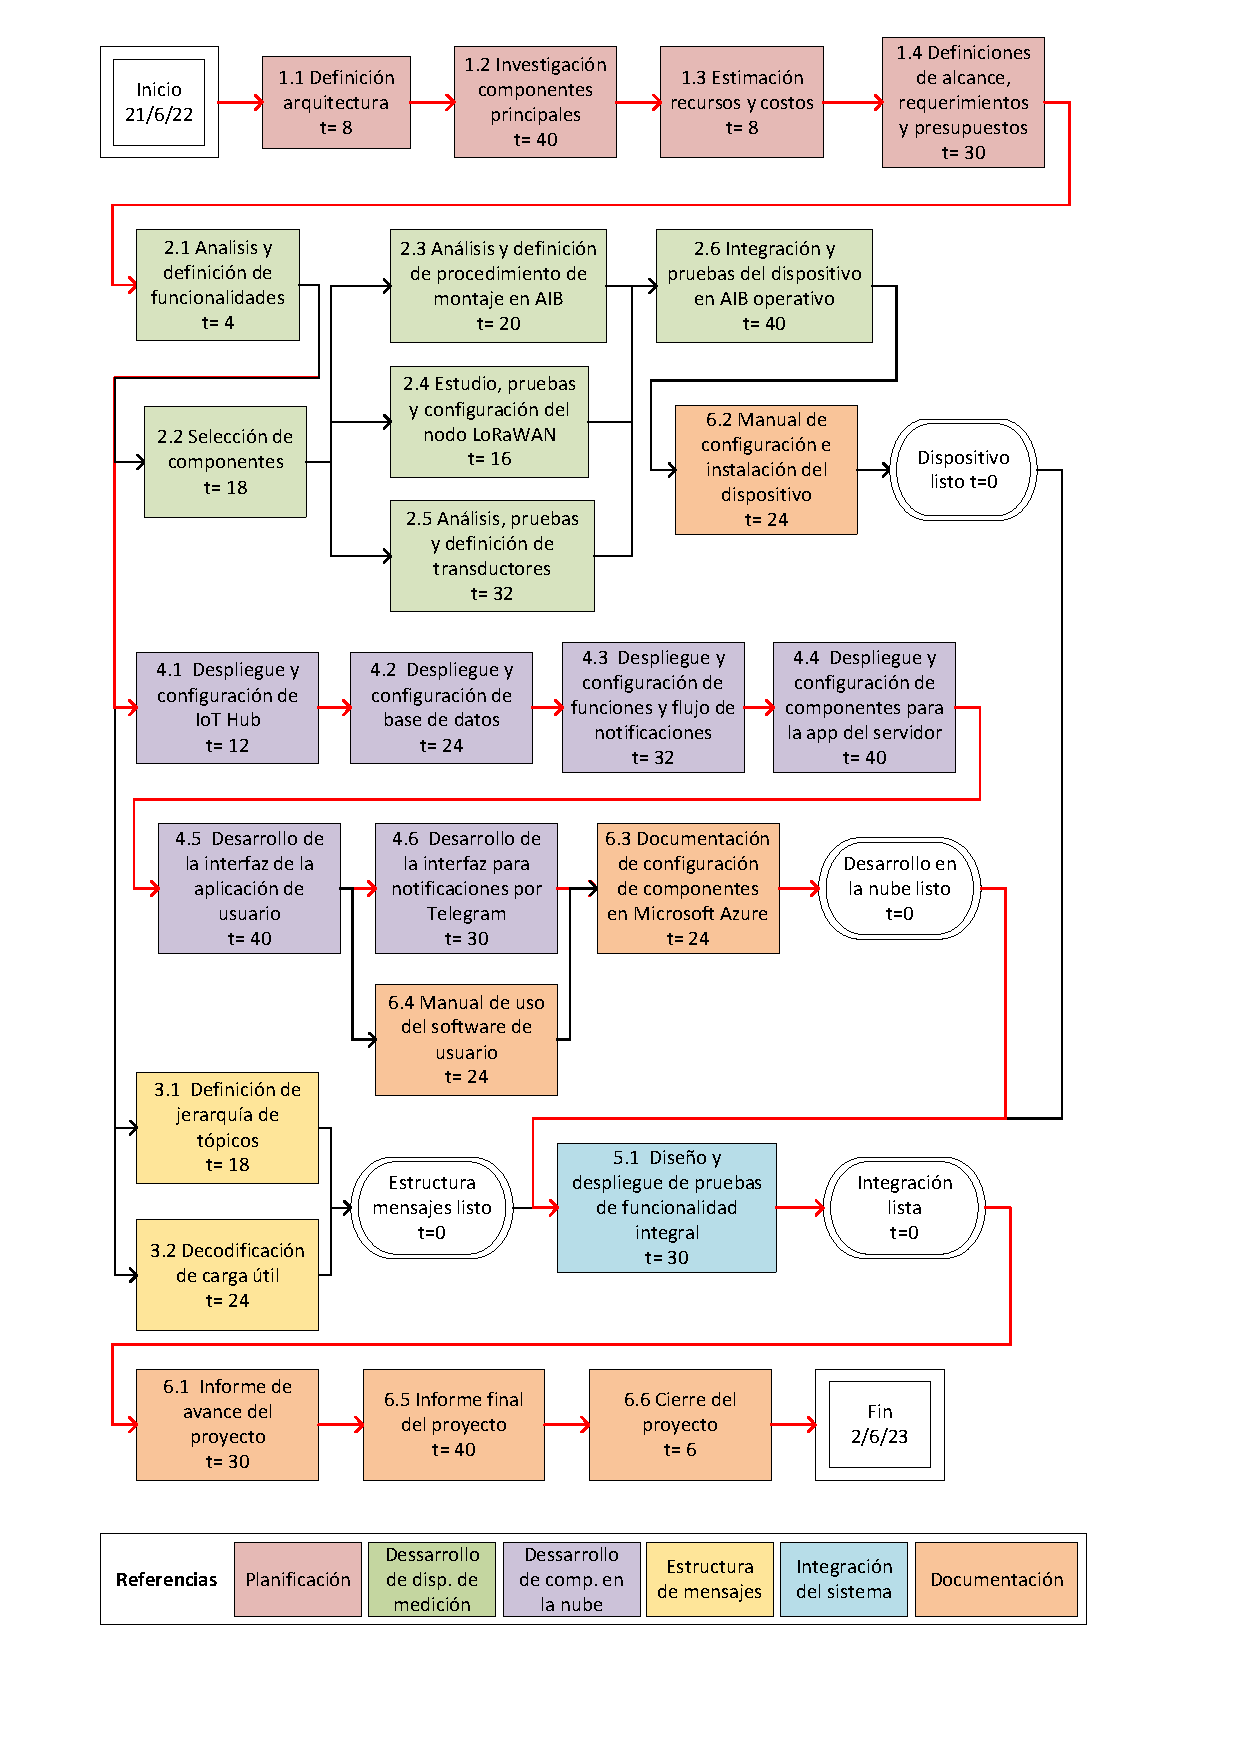
\includegraphics[width=1\textwidth]{./Figuras/Diagrama Activity on node_seleccion.pdf}
\caption{Diagrama en \textit{Activity on Node}.}
\label{fig:AoN}
\end{figure}



\section{11. Diagrama de Gantt}
\label{sec:gantt}

%\begin{consigna}{red}
%
%Existen muchos programas y recursos \textit{online} para hacer diagramas de gantt, entre los cuales destacamos:
%
%\begin{itemize}
%\item Planner
%\item GanttProject
%\item Trello + \textit{plugins}. En el siguiente link hay un tutorial oficial: \\ \url{https://blog.trello.com/es/diagrama-de-gantt-de-un-proyecto}
%\item Creately, herramienta online colaborativa. \\\url{https://creately.com/diagram/example/ieb3p3ml/LaTeX}
%\item Se puede hacer en latex con el paquete \textit{pgfgantt}\\ \url{http://ctan.dcc.uchile.cl/graphics/pgf/contrib/pgfgantt/pgfgantt.pdf}
%\end{itemize}

%Pegar acá una captura de pantalla del diagrama de Gantt, cuidando que la letra sea suficientemente grande como para ser legible. 
%Si el diagrama queda demasiado ancho, se puede pegar primero la ``tabla'' del Gantt y luego pegar la parte del diagrama de barras del diagrama de Gantt.
%
%Configurar el software para que en la parte de la tabla muestre los códigos del EDT (WBS).\\
%Configurar el software para que al lado de cada barra muestre el nombre de cada tarea.\\
%Revisar que la fecha de finalización coincida con lo indicado en el Acta Constitutiva.

%En la figura \ref{fig:gantt}, se muestra un ejemplo de diagrama de gantt realizado con el paquete de \textit{pgfgantt}. En la plantilla pueden ver el código que lo genera y usarlo de base para construir el propio.
%
%\begin{figure}[htbp]
%\begin{center}
%\begin{ganttchart}{1}{12}
%  \gantttitle{2020}{12} \\
%  \gantttitlelist{1,...,12}{1} \\
%  \ganttgroup{Group 1}{1}{7} \\
%  \ganttbar{Task 1}{1}{2} \\
%  \ganttlinkedbar{Task 2}{3}{7} \ganttnewline
%  \ganttmilestone{Milestone o hito}{7} \ganttnewline
%  \ganttbar{Final Task}{8}{12}
%  \ganttlink{elem2}{elem3}
%  \ganttlink{elem3}{elem4}
%\end{ganttchart}
%\end{center}
%\caption{Diagrama de gantt de ejemplo}
%\label{fig:gantt}
%\end{figure}

En la figura \ref{fig:diagWBS} se aprecia la tabla del desglose de actividades con sus fechas de inicio y fin, duración y asignación de recursos. Se identifican solo 2 recursos, el principal es el ejecutor (e) y el secundario es el colaborador (c).

En la figura \ref{fig:diagGantt} se muestra el diagrama de Gantt. Para la elaboración del mismo, se tomó una jornada de trabajo de 2,5 horas diarias, lo cual distribuye las 614 horas del proyecto en 346 días corridos. Se asume un esfuerzo continuo desde el inicio hasta el fin del proyecto, dedicándole los últimos dos meses exclusivamente a la elaboración de la memoria final.

En la sección anterior se realizó un diagrama AON donde se identificaron tareas que podían realizarse de forma simultánea y se determinó un camino crítico. La realidad es que al ser el ejecutor un único recurso, las tareas debieron reacomodarse de forma secuencial para reflejar ésta situación más realista.
%\begin{landscape}
\begin{figure}[htpb]
\centering 
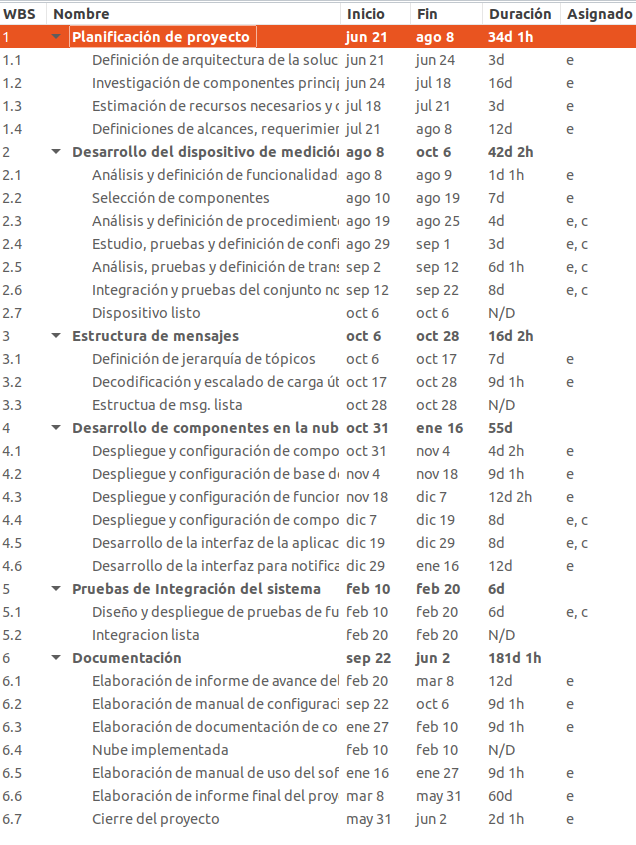
\includegraphics[height=.8\textheight]{./Figuras/wbs.png}
\caption{Desglose de actividades.}
\label{fig:diagWBS}
\end{figure}

%\end{landscape}

\begin{landscape}
\begin{figure}[htpb]
\centering 
\includegraphics[height=.9\textheight]{./Figuras/Gantt.png}
\caption{Diagrama de Gantt.}
\label{fig:diagGantt}
\end{figure}

\end{landscape}

%\end{consigna}


\section{12. Presupuesto detallado del proyecto}
\label{sec:presupuesto}


El presupuesto se expresa en pesos argentinos, tomando como referencia la fecha de inicio del proyecto.

Los costos directos mayormente lo conforman el valor de las horas de ejecución de las tareas detalladas.

Como estimación de los costos indirectos se considera un 40\% del total de costos directos. Forman parte de éstos licencias de software utilizadas, costos de servicios de comunicaciones, acceso a recursos informáticos de uso compartido, servicios de mantenimiento  mensual, gastos de transporte dentro del yacimiento y alquileres de oficinas y mobiliario.


\begin{table}[htpb]
\centering
\begin{tabularx}{\linewidth}{@{}|X|c|r|r|@{}}
\hline
\rowcolor[HTML]{C0C0C0} 
\multicolumn{4}{|c|}{\cellcolor[HTML]{C0C0C0}COSTOS DIRECTOS} \\ \hline
\rowcolor[HTML]{C0C0C0} 
Descripción &
  \multicolumn{1}{c|}{\cellcolor[HTML]{C0C0C0}Cantidad} &
  \multicolumn{1}{c|}{\cellcolor[HTML]{C0C0C0}Valor unitario} &
  \multicolumn{1}{c|}{\cellcolor[HTML]{C0C0C0}Valor total} \\ \hline
 Horas de desarrollo de ejecutor &
  
  \multicolumn{1}{c|}{614 h} &
  \multicolumn{1}{r|}{\$ 1500} &
  \multicolumn{1}{r|}{\$ 921.000} \\ \hline
 Horas de soporte de colaborador &
  \multicolumn{1}{c|}{109 h} &
  \multicolumn{1}{r|}{\$ 1500} &
  \multicolumn{1}{r|}{\$ 163.500} \\ \hline
\multicolumn{1}{|l|}{Cuadrilla de montaje en AIB} 
	& {16 h}
   & \multicolumn{1}{r|}{\$ 6.250}
   & \multicolumn{1}{r|}{\$ 100.000}
   \\ \hline
\multicolumn{1}{|l|}{Materiales: nodo, transductores y mat. menores} 
	& {1 u}
   & \multicolumn{1}{r|}{\$ 300.000}
   & \multicolumn{1}{r|}{\$ 300.000}
   \\ \hline
\multicolumn{1}{|l|}{Suscripción mensual de grupo recursos en Azure} 
	& {12 m}
   & \multicolumn{1}{r|}{\$ 5.000}
   & \multicolumn{1}{r|}{\$ 60.000}
   \\ \hline
\multicolumn{3}{|c|}{SUBTOTAL} &
  \multicolumn{1}{r|}{\$ 1.544.500} \\ \hline
\rowcolor[HTML]{C0C0C0} 
\multicolumn{4}{|c|}{\cellcolor[HTML]{C0C0C0}COSTOS INDIRECTOS} \\ \hline
\rowcolor[HTML]{C0C0C0} 
Descripción &
  \multicolumn{1}{c|}{\cellcolor[HTML]{C0C0C0}Cantidad} &
  \multicolumn{1}{c|}{\cellcolor[HTML]{C0C0C0}Valor unitario} &
  \multicolumn{1}{c|}{\cellcolor[HTML]{C0C0C0}Valor total} \\ \hline
%\multicolumn{1}{|l|}{} &
40\% de los costos directos
   & {1 u}
   & {\$ 617.800}
   & {\$ 617.800}
   \\ 
   \hline
%\multicolumn{1}{|l|}{} &
%   &
%   &
%   \\ \hline
%\multicolumn{1}{|l|}{} &
%   &
%   &
%   \\ \hline
%\multicolumn{3}{|c|}{SUBTOTAL} &
% \multicolumn{1}{c|}{} \\ \hline
\rowcolor[HTML]{C0C0C0}
\multicolumn{3}{|c|}{TOTAL} & \textbf{\$ 2.162.300}
   \\ \hline
\end{tabularx}%
\end{table}

\section{13. Gestión de riesgos}
\label{sec:riesgos}


a) Identificación de los riesgos y estimación de sus consecuencias:
 
Riesgo 1: Pérdida o sabotaje del dispositivo de medición.
\begin{itemize}
	\item Severidad (7): Generaría retrasos en el cronograma de implementación, ya que se deberían adquirir nuevamente los componentes y coordinar las tareas de montaje con cuadrillas operativas muy demandadas en el yacimiento.
	\item Probabilidad de ocurrencia (6): La pérdida por robo tiene una probabilidad cierta de ocurrencia, ya que el lugar seleccionado para la implementación del prototipo es un yacimiento de periferia con poca presencia de personas y bajo nivel de vigilancia.
\end{itemize}   

Riesgo 2: Falla de funcionamiento del dispositivo de medición al no soportar condiciones ambientales de operación.
\begin{itemize}
	\item Severidad (9): El dispositivo debe soportar condiciones climáticas extremas, altas vibraciones producidas por el sistema de bombeo mecánico y manipulación involuntaria en tareas de mantenimiento del equipamiento primario. Una falla de funcionamiento atribuida a estas causas, implicaría realizar un rediseño que pondría en riesgo la ejecución del proyecto. 
	\item Ocurrencia (3): Los componentes seleccionados cumplen exigentes condiciones ambientales, de todas maneras se identifica una probabilidad de falla ante la frecuente manipulación a la que pudieran estar expuestos.
\end{itemize}

Riesgo 3: Retraso en la asignación de recursos para el montaje del dispositivo de medición.
\begin{itemize}
	\item Severidad (4): Al igual que el riesgo 1, se generarían retrasos en el cronograma de implementación, comprometiendo los plazos acordados con el cliente.
	\item Ocurrencia (4): Existen situaciones imprevistas algo frecuentes que generan tareas de mayor prioridad para las cuadrillas de mantenimiento en el yacimiento.
\end{itemize}

Riesgo 4: No contar con el conocimiento necesario para desarrollar la aplicación de servidor e interfaz de usuario.
\begin{itemize}
	\item Severidad (7): No se dispone del conocimiento total requerido para su desarrollo en esta instancia del proyecto. Adquirirlos tardíamente podría demorar la ejecución del proyecto.
	\item Ocurrencia (3): Se contará con apoyo de un colaborador con mayor experiencia y los contenidos requeridos se asume que serán vistos en las materias de la especialización, por lo cual su probabilidad de ocurrencia es baja.
\end{itemize}

Riesgo 5: Cambio de proveedor de plataforma en la nube.
\begin{itemize}
	\item Severidad (8): Se debería adaptar la arquitectura y configuración de los componentes desarrollados para utilizarlos con las herramientas de otro proveedor. Tiene impacto en el costo de desarrollo y tiempo de implementación.
	\item Ocurrencia (1): Probabilidad baja, dado que existe relación comercial muy fuerte con el proveedor.
\end{itemize}

Riesgo 6: Cambio en la forma de facturación de los servicios consumidos en la nube.
\begin{itemize}
	\item Severidad (5): Podrían incrementarse los costos mensuales asumidos, afectando el presupuesto establecido.
	\item Ocurrencia (2):Probabilidad baja. Se contempla tener alternativas de implementación de los componentes o integración con otros grupos de recursos a fin de mantener los costos dentro de los límites establecidos.
\end{itemize}


Riesgo 7: Pérdida o daño de material de documentación.
\begin{itemize}
	\item Severidad (7): Afectaría los plazos de ejecución del proyecto, dado que se debería destinar tiempo adicional a su reelaboración.
	\item Ocurrencia (1): la notebook utilizada para su elaboración es de uso compartido para otras tareas laborales. Por ello, se utilizará un repositorio Git Hub y una rutina recurrente de actualización para minimizar el riesgo de ocurrencia.
\end{itemize}

b) Tabla de gestión de riesgos:      (El RPN se calcula como RPN = S x O)

\begin{table}[htpb]
\definecolor{miverde}{RGB}{118,215,196}
\definecolor{mirojo}{RGB}{214,148,138}
\centering
\begin{tabularx}{\linewidth}{@{}|X|c|c|c|c|c|c|@{}}
\hline
\rowcolor[HTML]{C0C0C0} 
Riesgo & S & O & RPN & S* & O* & RPN* \\ \hline
1. Pérdida o sabotaje del disp. de medición            & 7  & 6  & \cellcolor{mirojo}{42}    & 4 & 3 & \cellcolor{miverde}{12} \\ \hline
2. Falla de funcionamiento del disp. de medición       & 9  & 3  & \cellcolor{mirojo}{27}    & 7 & 1 & \cellcolor{miverde}{7}  \\ \hline
3. Retraso en la asignación de recursos para el montaje& 4  & 4  & \cellcolor{miverde}{16}   &  -  &  - &  -    \\ \hline
4. No contar con el conocimiento necesario             & 7  & 3  & \cellcolor{mirojo}{21}    & 3 & 3 & \cellcolor{miverde}{9}   \\ \hline
5. Cambio de proveedor de plataforma en la nube        & 8  & 1  & \cellcolor{miverde}{8}   &  -  &  -  & -     \\ \hline
6. Cambio en la forma de facturación de los servicios  & 5  & 2  & \cellcolor{miverde}{10}    & -   &  -  &  -  \\ \hline
7. Pérdida o daño de material de documentación         & 7  & 1  & \cellcolor{miverde}{7}   &  -  &  -  &  -    \\ \hline
\end{tabularx}%
\end{table}

Criterio adoptado: 
Se tomarán medidas de mitigación en los riesgos cuyos números de RPN sean mayores a 20

Nota: los valores marcados con (*) en la tabla corresponden luego de haber aplicado la mitigación.

c) Plan de mitigación de los riesgos que originalmente excedían el RPN máximo establecido:
 
Riesgo 1: Se dispondrá de un stock de al menos 3 unidades adicionales para contemplar reemplazos. Se notificará al sector de seguridad física de la empresa operadora de la realización del piloto, a fin de que se pueda instrumentar una rutina de vigilancia adicional.\\
Nueva asignación de S y O, con su respectiva justificación:
\begin{itemize}
	\item Severidad (4): Se reduce a un valor que contempla solo el retraso por la tarea de reinstalar el dispositivo.
	\item Ocurrencia (3): Se reduce la probabilidad al aumentar la disuasión por el incremento en la vigilancia.
\end{itemize}
 
Riesgo 2: Se supervisará el montaje del dispositivo de medición, de modo de evitar vicios de instalación. Se brindarán charlas de capacitación a las cuadrillas de mantenimiento al momento de realizar el montaje para evitar la incorrecta manipulación del dispositivo. Se realizará al menos una visita mensual para evaluar el estado de la instalación.\\
Nueva asignación de S y O, con su respectiva justificación:
\begin{itemize}
	\item Severidad (7): Con las medidas a adoptar, se tendrá un alerta temprana de alguna deficiencia en las prestaciones del dispositivo.
	\item Ocurrencia (1): Mitigando el factor humano de un mal uso o mala instalación, la probabilidad de falla se deberá únicamente a defectos de los componentes.
\end{itemize}
 
Riesgo 4: Al detectar el riesgo de desvío por demoras en la ejecución de tareas relacionadas a esta área de conocimiento, se solicitará asistencia de colaborador especialista. Se acordará previamente con la gerencia funcional del colaborador su afectación potencial al proyecto en un período específico de tiempo.\\
  Nueva asignación de S y O, con su respectiva justificación:
\begin{itemize}
	\item Severidad (3): Se reduce al contar con mayor respaldo para comenzar la tarea en el tiempo planificado.
	\item Ocurrencia (3): No se modifica.
\end{itemize}
 


\section{14. Gestión de la calidad}
\label{sec:calidad}

Se presentan a continuación los requerimientos con sus verificaciones y validaciones.

%\begin{itemize} 
%\item Req \#1: copiar acá el requerimiento.
%
%\begin{itemize}
%	\item Verificación para confirmar si se cumplió con lo requerido antes de mostrar el sistema al cliente. Detallar 
%	\item Validación con el cliente para confirmar que está de acuerdo en que se cumplió con lo requerido. Detallar  
%\end{itemize}

%\end{itemize}
%
%Tener en cuenta que en este contexto se pueden mencionar simulaciones, cálculos, revisión de hojas de datos, consulta con expertos, mediciones, etc.  Las acciones de verificación suelen considerar al entregable como ``caja blanca'', es decir se conoce en profundidad su funcionamiento interno.  En cambio, las acciones de validación suelen considerar al entregable como ``caja negra'', es decir, que no se conocen los detalles de su funcionamiento interno.
\begin{enumerate}
	\item Requerimientos asociados al dispositivo de medición.
		\begin{enumerate}
			\item No debe requerir mano de obra calificada, tanto para la instalación como para la operación cotidiana.
			\begin{itemize}
				\item Verificación: se comprobarán las instrucciones de montaje y operación.
				\item Validación: se supervisará la primera instalación del prototipo y la operación por un usuario designado.
			\end{itemize}

			\item Debe ser robusto y soportar condiciones de clima extremo (grado de protección IP 67, soportar temperaturas entre -20°C y 50°C).
			\begin{itemize}
				\item Verificación: se comprobarán los requisitos en las hojas de datos de los componentes.
				\item Validación: se inspeccionará la primera instalación del prototipo.
			\end{itemize}
			\item Debe funcionar con baterías internas y poseer una autonomía de al menos 3 años.
			\begin{itemize}
				\item Verificación: se comprobará la especificación de la batería del nodo y se realizará un cálculo de autonomía en función del caso de uso típico.
				\item Validación: se registrará un test de nivel de carga de batería en un intervalo de tiempo adecuado. 
			\end{itemize}
			\item La batería debe ser comercialmente asequible y de fácil reemplazo.
			\begin{itemize}
				\item Verificación: se inspeccionará esta característica en función de lo relevado en el mercado.
				\item Validación: se ofrecerá evidencia al cliente de las posibilidades de  asequibilidad en el mercado.  
			\end{itemize}
			\item El estado e información de los sensores del dispositivo se deben poder consultar mediante una aplicación inalámbrica desde un celular y de forma sencilla.
			\begin{itemize}
				\item Verificación: se comprobará esta funcionalidad en las hojas de datos del nodo.
				\item Validación: se ofrecerá realizar una prueba funcional al cliente.
			\end{itemize}
			\item Debe permitir el traslado a una nueva ubicación sin requerir una reconfiguración local.
			\begin{itemize}
				\item Verificación: funcionalidad propia de la tecnología de conexión seleccionada. No requiere una verificación explícita.
				\item Validación: se ofrecerá realizar una prueba funcional al cliente.
			\end{itemize}
			\item Debe detectar y notificar de forma inmediata si un sensor tiene una falla de cableado.
			\begin{itemize}
				\item Verificación: se comprobará el comportamiento del nodo al presentarse una condición de lazo abierto.
				\item Validación: se ofrecerá realizar una prueba funcional al cliente.
			\end{itemize}
		\end{enumerate}
		
	\item Requerimientos asociados a la colecta e identificación de mensajes generados por los dispositivos.
		\begin{enumerate}
			\item Se deberá definir un nomenclador de tópicos que sea flexible y escalable.
			\begin{itemize}
				\item Verificación: se revisará la forma de asignación de tópicos, planteando situaciones extremas.
				\item Validación: se realizará una prueba de definición de tópicos para distintos casos reales.
			\end{itemize}
			\item La estructura de la carga útil del mensaje debe soportar futuras  incorporaciones de sensores.
			\begin{itemize}
				\item Verificación: se comprobará la capacidad de incorporar nuevas variables a la carga útil del mensaje.
				\item Validación: se realizará prueba de modificación de carga útil y su correspondiente representación.
			\end{itemize}
		\end{enumerate}

	\item Requerimientos asociados al software en la nube.
		\begin{enumerate}
			\item Se deberán utilizar componentes de la plataforma Azure de Microsoft.
			\begin{itemize}
				\item Verificación: Se documentarán las características de cada componente de nube utilizado.
				\item Validación: no es requerida por el cliente.
			\end{itemize}
			\item Los mensajes de los dispositivos se enviarán a un componente IoT Hub mediante protocolo AMQP.
			\begin{itemize}
				\item Verificación: se tomarán muestras testigo de mensajes enviados.
				\item Validación: no es requerida por el cliente.
			\end{itemize}
			\item Se deberá decodificar y enrutar adecuadamente el flujo de datos proveniente de IoT Hub.
			\begin{itemize}
				\item Verificación: se tomarán muestras testigo de mensajes enviados.
				\item Validación: no es requerida por el cliente.
			\end{itemize}
			\item Se debe establecer un flujo de datos hacia una base de datos de históricos.
			\begin{itemize}
				\item Verificación: se harán consultas de prueba para verificar el correcto almacenamiento de información histórica.
				\item Validación: se dará acceso al cliente para verificar el almacenamiento de la información.
			\end{itemize}
			\item Se debe establecer un flujo de datos para procesar y enviar notificaciones de alarmas.
			\begin{itemize}
				\item Verificación: se comprobará el establecimiento del flujo de datos.
				\item Validación: se realizará una prueba de envío de notificaciones.
			\end{itemize}
			\item Se deberá definir un mecanismo de notificación de alarmas y eventos a los usuarios registrados. Podrá ser por email y/o Telegram.
			\begin{itemize}
				\item Verificación: se comprobará el establecimiento del flujo de datos.
				\item Validación: se realizará una prueba de envío de notificaciones.
			\end{itemize}
			\item La aplicación web dispondrá de un panel para visualizar información histórica de cada dispositivo.
			\begin{itemize}
				\item Verificación: se inspeccionará el acceso a la funcionalidad.
				\item Validación: se dará acceso al cliente para validar el panel de visualización de información histórica. 
			\end{itemize}
			\item La aplicación web permitirá la consulta de eventos y alarmas. Se debe recibir una notificación de forma inmediata ante un paro del motor.
			\begin{itemize}
				\item Verificación: se verificará la correcta activación de la notificación ante el evento de disparo.
				\item Validación: se realizará una prueba de funcionalidad simulada con el cliente.
			\end{itemize}
			\item Se deben recibir notificaciones de advertencia de nivel de batería bajo y algún otro parámetro que se identifique de utilidad, para realizar un correcto mantenimiento preventivo.
			\begin{itemize}
				\item Verificación: se inspeccionará la correcta notificación ante el evento de nivel de batería bajo.
				\item Validación: se realizará una prueba de funcionalidad simulada con el cliente.
			\end{itemize}
		\end{enumerate}

	\item Requerimientos de integridad y seguridad.
		\begin{enumerate}
			\item Se deberá establecer un mecanismo seguro de gestión y validación de usuarios de la aplicación web.
			\begin{itemize}
				\item Verificación: se comprobará la funcionalidad de gestión y validación de usuarios de la aplicación web.
				\item Validación: se realizará una demostración de uso de la aplicación web al cliente.
			\end{itemize}
			\item El acceso a la configuración de los dispositivos de medición estará protegido por un usuario y contraseña. Será utilizado únicamente por personal autorizado del sector TI de la empresa.
			\begin{itemize}
				\item Verificación: se compobará el proceso de alta del nodo en la red LoRaWAN.
				\item Validación: no es requerida por el cliente.
			\end{itemize}
		\end{enumerate}
	
	\item Requerimientos de documentación.
		\begin{enumerate}
			\item Se deberá elaborar el manual de configuración e instalación del dispositivo de medición.
			\begin{itemize}
				\item Verificación: se comprobará que la estructura y contenido sea el requerido. 
				\item Validación: se plantearán versiones preliminares a ser validadas por el cliente.
			\end{itemize}			
			\item Se deberá documentar la configuración de todos los componentes desplegados en Microsoft Azure.
			\begin{itemize}
				\item Verificación: se comprobará que la estructura y contenido sea el requerido. 
				\item Validación: se enviará al área de IT el entregable para su validación.
			\end{itemize}
			\item Se deberá elaborar el manual de uso del software de usuario.
			\begin{itemize}
				\item Verificación: se inspeccionará que la estructura y contenido sea el requerido.
				\item Validación: se plantearán versiones preliminares a ser validadas por el cliente.
			\end{itemize}
			\item Se deberá desarrollar el informe de avance del proyecto.
			\begin{itemize}
				\item Verificación: se generará progresivamente la documentación técnica de cada etapa del proyecto y se cumplirán los procesos requeridos para disponer del informe de avance conformado previo a la entrega.
				\item Validación: lectura, recepción de correcciones y sugerencias por parte del director del proyecto.
			\end{itemize}
			\item Se deberá desarrollar la memoria final del proyecto.
			\begin{itemize}
				\item Verificación: cierre de la documentación técnica de cada etapa del proyecto. 
				\item Validación: lectura, recepción de correcciones y sugerencias por parte del director del proyecto. Aprobación del taller de trabajo final.
			\end{itemize}
		\end{enumerate}
		
	\end{enumerate}

\section{15. Procesos de cierre}    
\label{sec:cierre}


Enmarcado en el proceso de cierre del proyecto se realizará una reunión formal de evaluación. La organización y conducción estará a cargo del responsable del proyecto. Deberán participar: el cliente, el impulsor y el orientador; quienes tendrán que registrar su evaluación a cada tema presentado. Podrán participar de forma opcional un representante de usuario final y los colaboradores.\\
A continuación, se detallan las actividades que se llevarán a cabo.
\begin{itemize}
	\item Evaluación del cumplimiento de las expectativas.
	\begin{enumerate}
		\item Se evaluará el grado de satisfacción del cliente con el resultado final del proyecto.
		\item Se evaluará el grado de cumplimiento de cada requerimiento.
		\item Se evaluará la ejecución del plan de trabajo, identificando si el mismo se cumplió dentro de los plazos establecidos. Si se identificaran desvíos, los mismos serán analizados en mayor detalle, para capturar oportunidades de mejora para nuevos proyectos.
		\item Se evaluará el grado de cumplimiento de la ejecución del presupuesto.  De manera análoga al punto anterior, si hubiera desvíos respecto al plan los mismos serán analizados y registrados.
		\item Se evaluará el grado de satisfacción con el cual los riesgos identificados originalmente (o no) fueron tratados en el proyecto.
	\end{enumerate}
	
	\item Finalización de la prestación de servicios.
	\begin{enumerate}
		\item Se dará cierre formal a las prestaciones de servicio y a la utilización de activos de la empresa que fueron reservados para la ejecución del proyecto.
	\end{enumerate}

	\item Archivo de la documentación del proyecto.
	\begin{enumerate}
		\item Se aprobará la documentación del proyecto, incluyendo las lecciones aprendidas. Se archivará en el repositorio oficial de la oficina de proyectos.
	\end{enumerate}

	\item Agradecimientos.
	\begin{enumerate}
		\item Se identificará y dará un reconocimiento a todos los participantes del proyecto, realizando una mención especial a quienes hayan tenido un rol protagónico o destacado. Se gestionará la publicación de un \textit{flyer} (volante digital) en la página principal de la intranet de la empresa, dando lugar a éste reconocimiento.
	\end{enumerate}


\end{itemize}

% Pautas de trabajo que se seguirán para analizar si se respetó el Plan de Proyecto original:
%	 - Indicar quién se ocupará de hacer esto y cuál será el procedimiento a aplicar. 
%	\item Identificación de las técnicas y procedimientos útiles e inútiles que se emplearon, y los problemas que surgieron y cómo se solucionaron:
%	 - Indicar quién se ocupará de hacer esto y cuál será el procedimiento para dejar registro.
%	\item Indicar quién organizará el acto de agradecimiento a todos los interesados, y en especial al equipo de trabajo y colaboradores:
%	  - Indicar esto y quién financiará los gastos correspondientes.


\end{document}
